% Licensed to the Apache Software Foundation (ASF) under one or more
% contributor license agreements. See the NOTICE file distributed with
% this work for additional information regarding copyright ownership.
% The ASF licenses this file to You under the Apache License, Version 2.0
% (the ``License''); you may not use this file except in compliance with
% the License. You may obtain a copy of the License at
%
% http://www.apache.org/licenses/LICENSE-2.0
%
% Unless required by applicable law or agreed to in writing, software
% distributed under the License is distributed on an ``AS IS'' BASIS,
% WITHOUT WARRANTIES OR CONDITIONS OF ANY KIND, either express or implied.
% See the License for the specific language governing permissions and
% limitations under the License.

\begin{changemargin}{1.5in}{0in}

\section{Overview}

The MetaCarta GTS appliance indexes documents and allows users to
search these documents based on both keywords and geographic
references. The MetaCarta Web Crawler allows system administrators
to configure connections and define jobs to ingest documents crawled
from web pages on the Internet.

This document specifies the means for crawling web pages, ingesting
content from those web pages, and maintaining the relationship between
your document index and those web pages.

\subsection{Assumptions}

This document assumes you have a basic level of familiarity with GTS
appliance administration. This document also assumes that you have a
basic understanding of the repositories to which you are trying to
connect. If you need more information about the MetaCarta GTS
appliance, please read the \documentref{MetaCarta GTS Administrator's
Guide} stored on the appliance at
\dirpath{/usr/share/doc/metacarta/AdminGuide.pdf}.

Throughout this document, we assume that your appliance is named \\
\url{metacarta.example.com}. 

\section{Installation}

The Web Crawler must be used with the MetaCarta Connector Framework,
described in the \documentref{Metacarta Connector Guide}. If you
already have the Connector Framework installed, you can install the
Web Crawler.  The Web Crawler is available as a field-test addon
ISO file from from Metacarta. Use the following steps to install the
Web Crawler to your appliance:

\begin{enumerate}

\item Confirm that the system is running correctly using
\command{check\_system\_health}.

\item Copy the disc image and md5sum supplied by MetaCarta to the
\dirpath{/isos} directory on your appliance. Rename the ISO file to
\dirpath{addon-web-conn.iso} when you copy it to your appliance.

\item Check the md5sum of the ISO file using the \command{md5sum} command.

\item Install the iso using the following command:

\command{upgrade\_control install /isos/addon-web-conn.iso}

The appliance will reboot once the installation is complete.

\item Upgrade your license file, if necessary, as described in
\documentref{MetaCarta Appliance Administrator's Guide}. You may need
to contact MetaCarta Customer Service to obtain the appropriate
license file. (Please see page \pageref{SupportContact} for contact
information.)
 
\end{enumerate}

\section{Configuration}

\subsection{Access to the Connector}

The administrator to the Web Crawler % Licensed to the Apache Software Foundation (ASF) under one or more
% contributor license agreements. See the NOTICE file distributed with
% this work for additional information regarding copyright ownership.
% The ASF licenses this file to You under the Apache License, Version 2.0
% (the ``License''); you may not use this file except in compliance with
% the License. You may obtain a copy of the License at
%
% http://www.apache.org/licenses/LICENSE-2.0
%
% Unless required by applicable law or agreed to in writing, software
% distributed under the License is distributed on an ``AS IS'' BASIS,
% WITHOUT WARRANTIES OR CONDITIONS OF ANY KIND, either express or implied.
% See the License for the specific language governing permissions and
% limitations under the License.

must have
access to the web interface at
\url{http://metacarta.example.com/crawler/}. In the default appliance
security setup, you must have a Basic Authentication account
configured for access to the Connector web interface at
\url{http://metacarta.example.com/crawler/}.  If you are not an appliance
administrator, please ask the appliance administrator to give you such
an account.

An appliance administrator can create an account with access to the
ingestion interface (in this case, username {\tt fred} and password
{\tt ginger}) by running the following command on the appliance:

\begin{console}
metacarta:\~{}\$ basic\_auth\_control add ingest\_users fred:ginger 
\end{console}

Depending on how you have configured authentication using the
\command{auth\_control} tool, you may need to make changes other than
adding yourself to the ingest\_users group. For more information on
security configuration and \command{auth\_control}, see the Security
Administration section of the \documentref{MetaCarta Appliance
Administrator's Guide}.



\section{Collecting Documents From The Web} % Retitle this, yo.

The Connector Framework manages retrieving documents from different
servers through \emph{jobs}. Jobs can be scheduled to run
regularly; each job connects to a server using a particular
set of credentials. Each job is tied to a \emph{repository
connection}. Repository connections contain information allowing the
connector framework to connect to a given repository. A repository
connection may be tied to an \emph{authority connection}, which
manages document security. While using the Web Crawler to connect
to web pages, no authority connection is needed; you can simply
create a repository connection.


\subsection{Creating Repository Connections}

In order to create jobs to ingest documents, you need to create a
repository connection. To do so, click ``List Repository
Connections'' on the sidebar menu. Then, when presented with the list
of repository connections, click ``Add a new connection.'' You will
see the following two tabs:


% Licensed to the Apache Software Foundation (ASF) under one or more
% contributor license agreements. See the NOTICE file distributed with
% this work for additional information regarding copyright ownership.
% The ASF licenses this file to You under the Apache License, Version 2.0
% (the ``License''); you may not use this file except in compliance with
% the License. You may obtain a copy of the License at
%
% http://www.apache.org/licenses/LICENSE-2.0
%
% Unless required by applicable law or agreed to in writing, software
% distributed under the License is distributed on an ``AS IS'' BASIS,
% WITHOUT WARRANTIES OR CONDITIONS OF ANY KIND, either express or implied.
% See the License for the specific language governing permissions and
% limitations under the License.

\begin{picture}(1,1)
  \put(-100,15){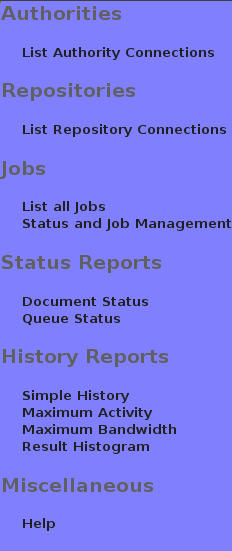
\includegraphics[width=80pt]{crawler-sidebar}}
\end{picture}



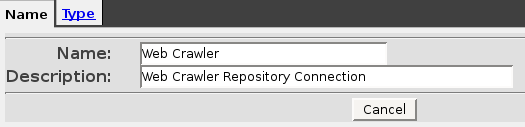
\includegraphics[width=300pt]{web-edit-repository-tab1}

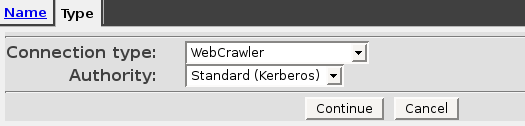
\includegraphics[width=300pt]{web-edit-repository-tab2}

Now you must provide a name, description, and connector type for your
new repository connection. The name should be unique, as you will use
it to select this connection later when defining jobs. The description
should explain the repository connection to you or another
administrator.  The connector type is the type of repository from
which you will get documents, in this case a Web Crawler. The
authority type is the type of authority from which you will get
authorization information. The Web Crawler does not use an
administrator-created authority; you should simply select ``Standard
(Kerberos)'' here.

Once you have filled in those tabs, click Continue to be taken to the
repository-specific options.

% Licensed to the Apache Software Foundation (ASF) under one or more
% contributor license agreements. See the NOTICE file distributed with
% this work for additional information regarding copyright ownership.
% The ASF licenses this file to You under the Apache License, Version 2.0
% (the ``License''); you may not use this file except in compliance with
% the License. You may obtain a copy of the License at
%
% http://www.apache.org/licenses/LICENSE-2.0
%
% Unless required by applicable law or agreed to in writing, software
% distributed under the License is distributed on an ``AS IS'' BASIS,
% WITHOUT WARRANTIES OR CONDITIONS OF ANY KIND, either express or implied.
% See the License for the specific language governing permissions and
% limitations under the License.

\subsubsection{Configuring a Web Crawler}

You must fill in the following tabs if you are configuring a Web Crawler:

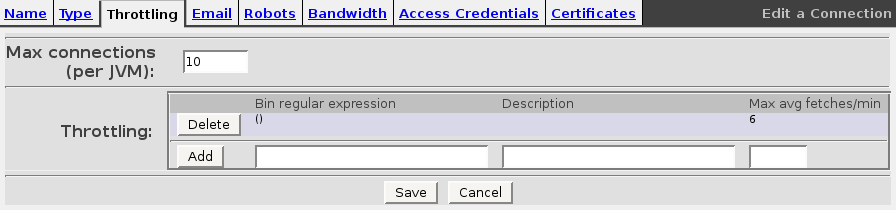
\includegraphics[width=300pt]{web-edit-repository-tab3}

\begin{itemize}

\item \textbf{Max connections (per JVM):} Here you can set the
maximum number of connections to your repository. For the Web Crawler,
you should increase the number of connections from the default 10 to
100. Configuration of other sections on this tab and the ``Bandwidth''
tab allow you to limit the number of connections to individual servers;
increasing the number here helps ensure that the crawler is able to take
full advantage of multiple throttling groups, which are explained below.


\item \textbf{Throttling:} Here you can set a maximum average document fetch
rate for the repository connection. The maximum fetch rate allows you
to set three things: Expression, description, and fetches per minute.

In the Web Crawler, the bin expression for a document is the name of
the server that hosts it. For example, if a document's URL is
\url{http://www.example.com/index.html}, the bin expression
associated with the document is \texttt{www.example.com}.  You can
create regular expressions to match the bin expression. The example
given here, \texttt{()}, matches all expressions, and thus throttles
all documents together. We recommend a maximum average rate of 6
fetches per minute.  Once you have set an expression, description, and
rate, click Add.

% Can you say what the expression is? I can't read it in the picture
% and I even have pretty good eyes :) 

\end{itemize}

In general, you should be conscientious about document fetch rates,
download rates, and other rates related to server traffic when using
the Web Crawler to connect to servers on the open Internet. The
recommended rates suggested in this guide are typically an upper
limit. You should not exceed these suggestions when crawling servers
on the open Internet. Higher demands on these servers may produce
undesirable effects in their performance; the administrators of those
servers may block your connection.

% We capitalize this more often than we don't; I will fix it everywhere.

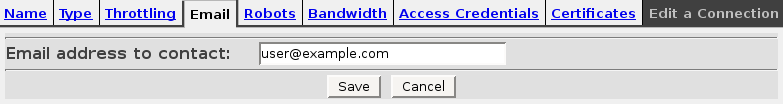
\includegraphics[width=300pt]{web-edit-repository-tab4}

\begin{itemize}

\item \textbf{Email:} A contact email address. This email address is included in request headers sent to servers. Administrators of servers recieving these requests may wish to contact you regarding your interactions with their content servers.

\end{itemize}

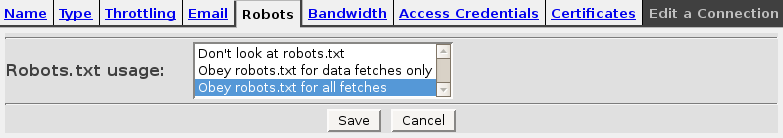
\includegraphics[width=300pt]{web-edit-repository-tab5}

\begin{itemize}

\item \textbf{Robots.txt Usage:} This determines whether the crawler obeys guidelines from the \dirpath{robots.txt} file on a server. There are three options:

\begin{itemize}

\item \textbf{Don't look at robots.txt}

\item \textbf{Obey robots.txt for data fetches only}

\item \textbf{Obey robots.txt for all fetches}

\end{itemize}

By default, \textbf{Obey robots.txt for all fetches} is selected. When
selected, the crawler will obey all interfacing and downloading
guidelines set in a server's \dirpath{robots.txt} file. You should
always use this setting when connecting to servers on the open
Internet.

\end{itemize}

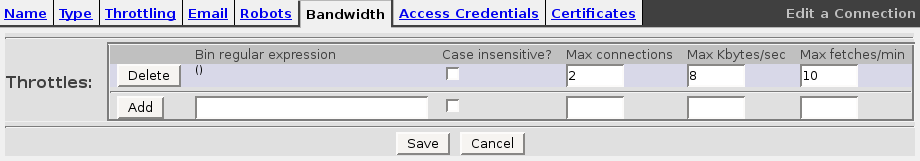
\includegraphics[width=300pt]{web-edit-repository-tab6}

On this tab, you can create throttling groups to limit maximum
connection, download, and fetch rates.

\begin{itemize}


\item \textbf{Throttles}:

\begin{itemize}

\item \textbf{Bin regular expression}: A regular expression to match the bins, as described previously.

\item \textbf{Case insensitive?} Should the match expression be case insensitive?

\item \textbf{Max connections}: The maximum number of connections to for each throttle group. This should be 1 or 2 for servers on the open Internet.

\item \textbf{Max Kbytes/sec}: The maximum download rate for each throttle group. This should be no more than 8 kilobytes per second for servers on the open Internet.

\item \textbf{Max fetches/minute}: The maximum number of document fetches per minute for each throttle group. This should be no higher than 10 fetches per minute for servers on the open Internet.

\end{itemize}

\end{itemize}

The set of all throttle groups you create should cover all the servers
that will be crawled through this repository connection. The easiest
way to ensure that you are limiting all server traffic is to create a
throttling group with the expression \texttt{()} and the appropriate
traffic limits, as shown in the picture above.

\bigimage{web-edit-repository-tab7}


On this tab, you can provide credentials for the crawler to use when
crawling servers protected by basic authentication or NTLM.

\begin{itemize}

\item \textbf{Access Credentials:} 

\begin{itemize}

\item \textbf{URL regular expression}:
Here you can specify a regular expression based on URL. If the crawler
requires credentials when attempting to crawl a document with a
matching URL, it will use the credentials supplied in the following
fields.

\item \textbf{Authorization type}: Select NTLM authentication or basic authentication. (Only LM and NTLMv1 are supported at this time.)

\item \textbf{Domain}: Here you can specify the NTLM domain that will be supplied as part of the user name credentials. Only required if you selected NTLM authentication.

\item \textbf{User name}: The user name that the crawler will use to connect.

\item \textbf{password}: (Optional) The password corresponding with that user name.

\end{itemize}

\end{itemize}

Click the ``Add'' button to include the specified credentials. You can
add multiple sets of credentials.

\missing{The main new feature for this release, see notes in graph paper, will need more screenshots}

\bigimage{web-edit-repository-tab8}

\begin{itemize}

\item \textbf{Trust certificates:}
In some cases, the crawler may need SSL certificates to access certain
content. You can upload SSL certificates here. This is dependent on
the configuration of the servers hosting the crawled content.  The
repository connection will need certificates similar to those used to
connect to the documents using an Internet browser.


If the certificate authority used to sign the content server's
certificate is a well-known authority, you will not need to upload a
certificate here; the appliance will automatically accept a
certificate from the server. If the server certificate is signed by an
unknown authority, you should upload the authority's certificate. In
some cases, the authority may be unavailable. In this case, you can
upload the server-side certificate itself. Server-side certificate
changes may require you to upload newer versions of this certificate
if you use this option.



\end{itemize}

After entering this information, you will be taken to the repository
connection status page for this repository:

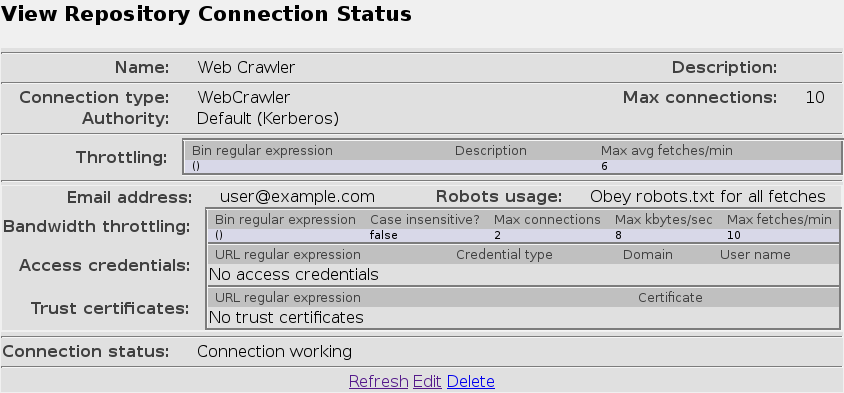
\includegraphics[width=300pt]{web-view-repo-conn-status}

In this example (which does not contain accurate information for any Web
Connector), the Connection Status is ``Connection working.''  If the
Connection Status is ``Connection failed,'' the web sites you want to
crawl might be down. Alternately, you might have incorrectly entered
data in one of the fields; if so, click ``Edit'' to fix the data.


\subsection{Creating and Running Jobs}

To run a job, click ``Status and Job Management'' on the sidebar menu.
You can run or edit existing jobs from this menu.

To create a new job, click ``List All Jobs'' on the sidebar menu. Then, when
presented with the list of current jobs, click ``Add a new job.'' You
will be presented with two tabs, in which you must fill in the following
information:

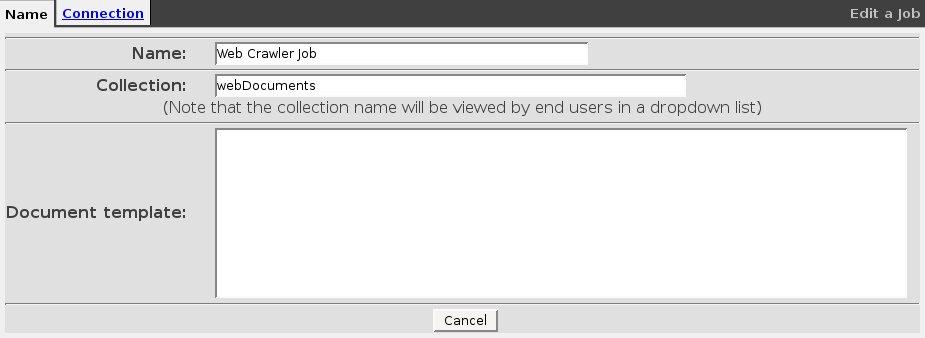
\includegraphics[width=300pt]{web-edit-job-tab1}

\begin{itemize}

\item \textbf{Name:} The name of the job. You will use this to identify
the job later.

\item \textbf{Collection:} The collection name metadata for all
documents in this job. End users can use this name to select the set
of documents in this job. For more information on collection name
metadata, please see the \documentref{MetaCarta GTS Administrator's
Guide}.

\item \textbf{Document template:} % Licensed to the Apache Software Foundation (ASF) under one or more
% contributor license agreements. See the NOTICE file distributed with
% this work for additional information regarding copyright ownership.
% The ASF licenses this file to You under the Apache License, Version 2.0
% (the ``License''); you may not use this file except in compliance with
% the License. You may obtain a copy of the License at
%
% http://www.apache.org/licenses/LICENSE-2.0
%
% Unless required by applicable law or agreed to in writing, software
% distributed under the License is distributed on an ``AS IS'' BASIS,
% WITHOUT WARRANTIES OR CONDITIONS OF ANY KIND, either express or implied.
% See the License for the specific language governing permissions and
% limitations under the License.

You may also input a document template. A document template, written
in XML, limits the parts of the document that are indexed.  Simply
input the XML in the text entry field.  For information on how to
construct a document template, please see the \documentref{MetaCarta
Document Templates Integrator's Guide}.


\end{itemize}

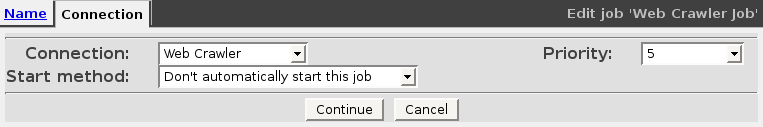
\includegraphics[width=300pt]{web-edit-job-tab2}

\begin{itemize}

\item \textbf{Connection:} The name of the repository connection you
wish to use for this job. You select this from the list of repository
connections you have already made. You may have more than one job use
the same repository connection, but if you have two jobs crawl the same
documents, the documents will have the metadata and collection name
associated with whatever job crawled the document most recently. This
will cause unpredictable results when searching those collections,
searching for those documents, or trying to delete those collections.
We recommend never crawling the same document in two different jobs.

\item \textbf{Start method:} Whether you want to start this job the next
time jobs are scheduled to run (``Start when schedule window starts''),
immediately after you finish defining it (``Start even inside a schedule
window''), or not at all (``Don't automatically start this job'').

\item \textbf{Priority:} From 1 (highest) to 10 (lowest), the priority
this crawl should have if it must compete for resources with other
crawls on the appliance. You should not need to change this unless you
are running more than one crawl at the same time; if you are, assign a
higher priority to the crawls whose documents you want to be processed
preferentially before documents from other jobs.

\end{itemize}

After filling in those options, click ``Continue'' and you will be
presented with two additional repository-specific tabs.

% Licensed to the Apache Software Foundation (ASF) under one or more
% contributor license agreements. See the NOTICE file distributed with
% this work for additional information regarding copyright ownership.
% The ASF licenses this file to You under the Apache License, Version 2.0
% (the ``License''); you may not use this file except in compliance with
% the License. You may obtain a copy of the License at
%
% http://www.apache.org/licenses/LICENSE-2.0
%
% Unless required by applicable law or agreed to in writing, software
% distributed under the License is distributed on an ``AS IS'' BASIS,
% WITHOUT WARRANTIES OR CONDITIONS OF ANY KIND, either express or implied.
% See the License for the specific language governing permissions and
% limitations under the License.

\subsubsection{Web Crawler Job Options}

You must fill in six more tabs to configure a Web Crawler job.

\bigimage{web-edit-job-tab3}

\ifJDBCGuide
% Licensed to the Apache Software Foundation (ASF) under one or more
% contributor license agreements. See the NOTICE file distributed with
% this work for additional information regarding copyright ownership.
% The ASF licenses this file to You under the Apache License, Version 2.0
% (the ``License''); you may not use this file except in compliance with
% the License. You may obtain a copy of the License at
%
% http://www.apache.org/licenses/LICENSE-2.0
%
% Unless required by applicable law or agreed to in writing, software
% distributed under the License is distributed on an ``AS IS'' BASIS,
% WITHOUT WARRANTIES OR CONDITIONS OF ANY KIND, either express or implied.
% See the License for the specific language governing permissions and
% limitations under the License.

\begin{itemize}
\label{scheduling}

\item \textbf{Schedule type:} Whether you want to scan every document
once or dynamically recrawl content in your repository. 

When scanning every document once, the crawler marks all documents that
have been previously crawled in this job as potentially to be deleted,
adds all seed documents to its queue and marks them as pending, processes
pending documents, marking them completed as they are ingested, and then
deleted all of the documents that were not recrawled. A document might
not be recrawled because it no longer exists, or the job specification
might have been changed to no longer include the document.

When dynamically recrawling documents, the crawler does not start by
marking all documents as potentially deletable; instead, it begins with
all of the seed documents, and continues adding to its list, periodically
re-adding the initial seed documents. If a document is removed from the
source, it will expire in the expiration interval (see below).

\item \textbf{Expiration Interval (if continuous):} The length of the
interval (in minutes) that the appliance will retain a document
crawled by this job after the document no longer appears in the
repository. After this interval, the missing document will be removed
from the appliance's index and archive. Leave the expiration interval
blank to keep missing documents indexed in GTS.

\item \textbf{Recrawl interval:} If you are dynamically recrawling
documents, how long, in minutes, the crawler should wait before
crawling documents a second time.

\item \textbf{Reseed interval:} If you are dynamically recrawling
documents, how long, in minutes, the crawler should wait before
looking for new documents to crawl. \ifMeridioGuide This connector
identifies all documents for ingestion through seeding; if the reseed
interval is infinite, the job will not ingest documents placed in the
repository during run time. (The job automatically reseeds whenever it
is started.) The default interval of 60 minutes is an appropriate
reseed rate. \fi \ifFilenetGuide This connector identifies documents
for ingestion during seeding. If you change the document inclusion
criteria, reseeding is required to identify new documents. Similarly,
documents placed in the repository while the job is running will not
be identified until the crawl is reseeded.  (The job automatically
reseeds whenever it is started.) The default interval of 60 minutes is
an appropriate reseed rate. \fi

\item \textbf{Scheduled time:} Allows you to define a time you wish
the job to run using a series of selection boxes. The first box refers
to the day of the week you wish the job to run, with an option to have
the job run any day of the week. The second box allows you to select
the start hour, with an option to start the job at any hour. The third
box allows you to specify which minute after the hour that you wish
the job to start. The fourth box allows you to specify what months of
the year you wish the job to run, with an option for the job to run
any month. The last box allows you to specify the day of the month you
wish the job to start, including any day of month.


You can scroll through each of the five boxes in this setting using
the arrow keys on your keyboard or by using the scroll bar on the
right side of the box.  If you want to select more than one value,
hold down control as you scroll and click the values that you want to
select. This allows you to define multiple windows with the same
length, for example by selecting Monday, Wednesday, and Friday at the
same time.

\item \textbf{Maximum run time:} The longest you will allow the job to
run, in minutes. For example, if you want to start a job at 2 AM but
force it to stop at 8 AM so that users have access to the repository,
you should set this value to 360 minutes. If the job is not complete by the
end time, documents that have already been found will be indexed, and
the rest of the crawl will continue at the beginning of the next
schedule interval. 

When you have defined the scheduled time and assigned a maximum run
time, click on the ``Add Scheduled Time'' button. A new schedule box
will appear below the scheduled time, allowing you to create
additional scheduled run times.

Here is a sample schedule for a job that will run every
Monday from 2 am to 6 am:

\begin{changemargin}{-.3in}{0in} 
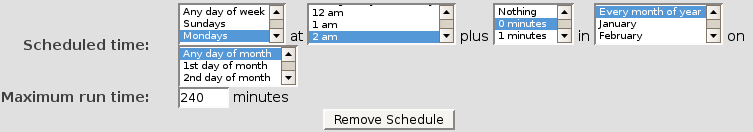
\includegraphics[width=300pt]{sample-schedule}
\end{changemargin}

If you do not have at least one scheduled time, the job will
only run when run manually (see page \pageref{ManageJobs}), and will
not automatically update the index on the appliance based on changes
to the repository.

You can remove a scheduled time by clicking the ``Remove Schedule''
button.

\end{itemize}

\fi

\ifCombinedConnectorGuide
This tab presents scheduling options. Here you can generate one or
more scheduled run times for the job. For a complete description of
the scheduling options, see the description starting on page
\pageref{scheduling}.
\fi

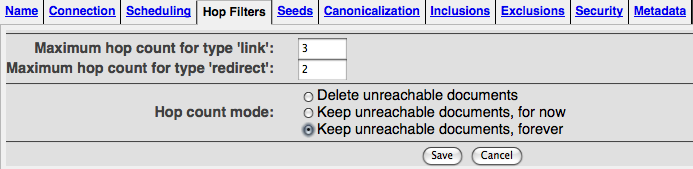
\includegraphics[width=300pt]{web-edit-job-tab4}

\begin{itemize}

\item \textbf{Maximum hop count for type 'link':} The web crawler begins
at the seed documents provided on the following tab, and follows links
in the bodies of the documents, if applicable.  Only documents where
the crawler follows this number or fewer links to reach that document
from a seed document will be processed.


\item \textbf{Maximum hop count for type 'redirect':} The maximum hop
count for type 'redirect' limits which documents will be processed by
the crawl based on the number of redirect links between that document
and a seed document.

\item \textbf{Hop count mode:} Documents may become unreachable within the
limiting number of hops from the seed documents. This setting determines
how documents that become unreachable are treated in the database.

\begin{itemize}

\item \textbf{Delete unreachable documents}:
Documents that become unreachable from the seed pages in the number of
hops specified above will be deleted from the database. Deleting
unreachable documents may affect resources available on the appliance.

\item \textbf{Keep unreachable documents, for now}:
When the crawler attempts to re-crawl a document and finds it
unreachable, the documents are kept. You can decide at any point later
to keep these documents forever or to delete them, by changing this
setting. Some appliance resources will be used to maintain the status
of these documents.

% What kinds of resources? Disk? RAM? Sheep?

\item \textbf{Keep unreachable documents forever}:
Documents that are unreachable are kept in the document index. You
cannot delete these documents from the index without deleting the job
used to crawl the documents. This is the preferred setting.

\end{itemize}

\end{itemize}


\bigimage{web-edit-job-tab5}

On this tab, you are presented with a text box into which you should
enter the URLs of the web pages you wish this job to crawl. Each
should be on a separate line of the text box.

\bigimage{web-edit-job-tab6}

This tab allows you to apply some built-in canonicalization tools
to URLs before they are send to the MetaCarta ingestion system. If
canonicalization is not done properly, you risk either having duplicate
copies of the same document (for example, from having arguments to
a script in a different order but calling the script with the same
arguments) or having no copies of a document at all (for example, from
reordering the script arguments in a way that breaks the site being
crawled). The Connector Framework handles the reordering automatically,
but requires your intervention to decide which sites need to be reordered
and which do not.

You can canonicalize based on regular expression; for more information on
regular expressions, please see the explanation in the next tab. Enter
a regular expression, a description of the URL (for your records only),
and then choose the types of canonicalization you would like enabled. You
have the following canonicalization options:

\begin{itemize}

\item \textbf{Reorder}: Take all arguments to any query in the URL and
order them programmatically. For example, a URL might include a query
string like ``article=foo0011\&format=fulltext.'' If the query string
were instead ``format=fulltext \&article=foo0011,'' the MetaCarta system
would treat it as a different document but it would contain the same
information. Normally, we recommend that you reorder all URLs, but
some sites require a specific order; for those sites, you should turn
reordering off.

\item \textbf{Remove JSP sessions}: Most of the time, you can safely
remove JSP session information from URLs. Uncheck this box if you find
that a particular site requires that you leave JSP session information
in the URL.

\item \textbf{Remove ASP sessions}: Most of the time, you can safely
remove ASP session information from URLs. Uncheck this box if you find
that a particular site requires that you leave ASP session information
in the URL.

\item \textbf{Remove PHP sessions}: Most of the time, you can safely
remove PHP session information from URLs. Uncheck this box if you find
that a particular site requires that you leave PHP session information
in the URL.

\item \textbf{Remove BV sessions}: Most of the time, you can safely
remove BV session information from URLs. Uncheck this box if you find
that a particular site requires that you leave BV session information
in the URL.

\end{itemize}

By default, all URLs are canonicalized in all five ways.

\bigimage{web-edit-job-tab7}


Here you can create regular expression matches that will determine
what the crawler includes for ingestion based on URL.  Place each
inclusion expression on a new line in the text box.

The default expression, \texttt{.*}, includes all documents. If you
are crawling the open Internet, this may cause your crawl to follow
links from and ingest many undesirable documents. A better strategy
may be to create expressions that match individual servers or
domains. In the example above, the given match expression\linebreak
\texttt{\^{}https?://[\^{}$\backslash\backslash\backslash$?/]*.example.com} only matches documents from the\linebreak \texttt{example.com} domain.

\note{If you are not familiar with regular expressions, there
are a variety of tutorials available on the web, including
\url{http://gnosis.cx/publish/}\linebreak\url{programming/regular_expressions.html}
and \url{http://perldoc.}\linebreak\url{perl.org/perlrequick.html}. If you still have
difficulty with these settings, please contact Customer Support (see
page \pageref{SupportContact}).}


\bigimage{web-edit-job-tab8}


Here you can create regular expression matches that will determine
what the crawler excludes from ingestion. Place each exclusion
expression on a new line in the text box.

The default blank expression does not exclude any documents. Other
possiblities include specifying specific servers or domains to
exclude. For example, the match expression
\texttt{\^{}https?://media.example.com} excludes any documents from
the \texttt{media.example.com} server. Another possibility is to
exclude files based on file extension. For example, the match
expression \texttt{$\backslash$.exe($\backslash$?|\$)} will exclude any
file with a \texttt{.exe} extension.


\bigimage{web-edit-job-tab9}



\begin{itemize}

\item \textbf{Access Tokens:} If you wish to create ACLs for files
ingested through this job, you can enter access tokens here. Simply
enter one or more ACL identifiers into the field and click the ``Add''
button. The ACL identifiers will appear in a list. You can continue to add
more ACL identifiers using the ``Add'' button, or remove them using the
``Delete'' button that appears next to each ACL identifier. By default,
documents ingested through the Web Crawler will be accessible to all
authorized search users. For assistance with this configuration, contact
MetaCarta Support (see page \pageref{SupportContact}).

%% don't we explain this in other guides? It would be nice to explain it, I think... 

\end{itemize}


\bigimage{web-edit-job-tab10}


\begin{itemize}

\item \textbf{Metadata:} Here you can add additional metadata to be ingested along with documents crawled by this job. You should not overwrite existing metadata fields, such as collection name, using this tool.

\end{itemize}

After entering this information, you will be taken to the status page
for this job:

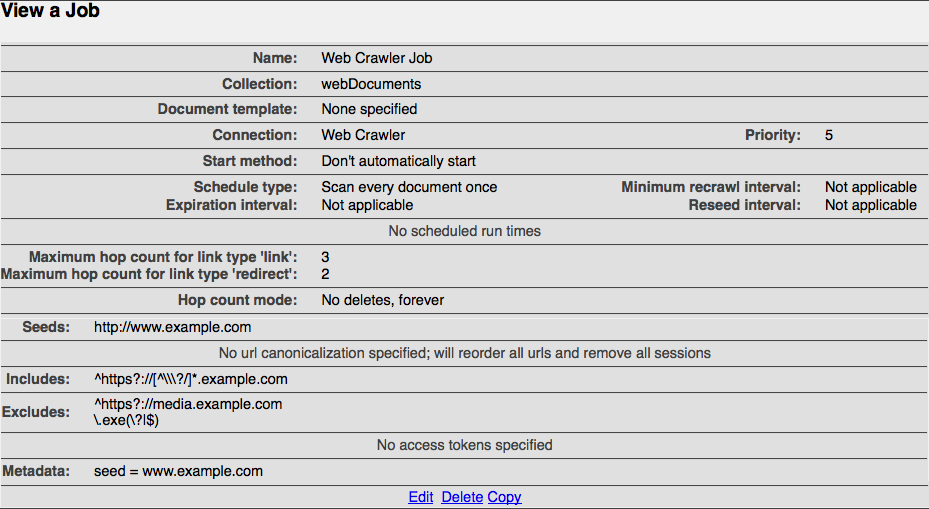
\includegraphics[width=300pt]{web-view-job-status}


\subsection{\label{ManageJobs}Status and Job Management}

You can then look at the status of your job by clicking ``Status and 
Job Management'' on the sidebar. You will see a list of one or more jobs
much like this one:

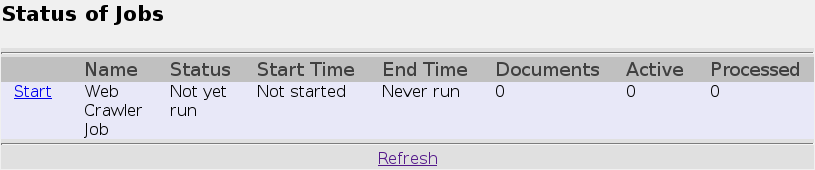
\includegraphics[width=300pt]{web-jobs-list}

You can start any crawl you like immediately from this interface by
clicking ``Start'' next to the name of the crawl. This interface also
allows you to see how many documents have been crawled; this information
may help you structure and plan future crawls.

\note{Refresh this page by clicking the ``Refresh'' link at the bottom
of the page, not by clicking your browser's reload button.}

\section{Tuning Crawl Peformance}

During high broad, high intensity crawls, you may wish to tune your
crawl by changing the number of threads dedicated to ingestion. In the
file \dirpath{/etc/metacarta/agents.conf} on your appliance, you
can change the \texttt{com.metacarta.crawler}\linebreak\texttt{.threads} parameter from
its default value of 30 up to 80. Dedicating more appliance resources
to the crawl can help the crawl complete faster. However, it may
affect other aspects of appliance performance.

% Like what? We should at least give an overview, I think. Maybe
% "including search UI responsiveness" at least...


\section{Reports}

The Connector interface can generate two types of status reports, on
current crawl status, and four types of history reports, on past crawl
history.

\subsection{Status Reports}

The two types of status report are:

\begin{itemize}

\item Document Status, which lets you find information on individual
documents currently part of a job.

\item Queue Status, which lets you aggregate information about groups
of documents currently part of a job.

\end{itemize}

\subsubsection{Document Status}

This report was generated by selecting ``Web Crawler,'' selecting the document state ``Documents processed at
least once,'' selecting all possible document statuses, clicking
continue, selecting ``WebCrawlerJob,'' and clicking Go.

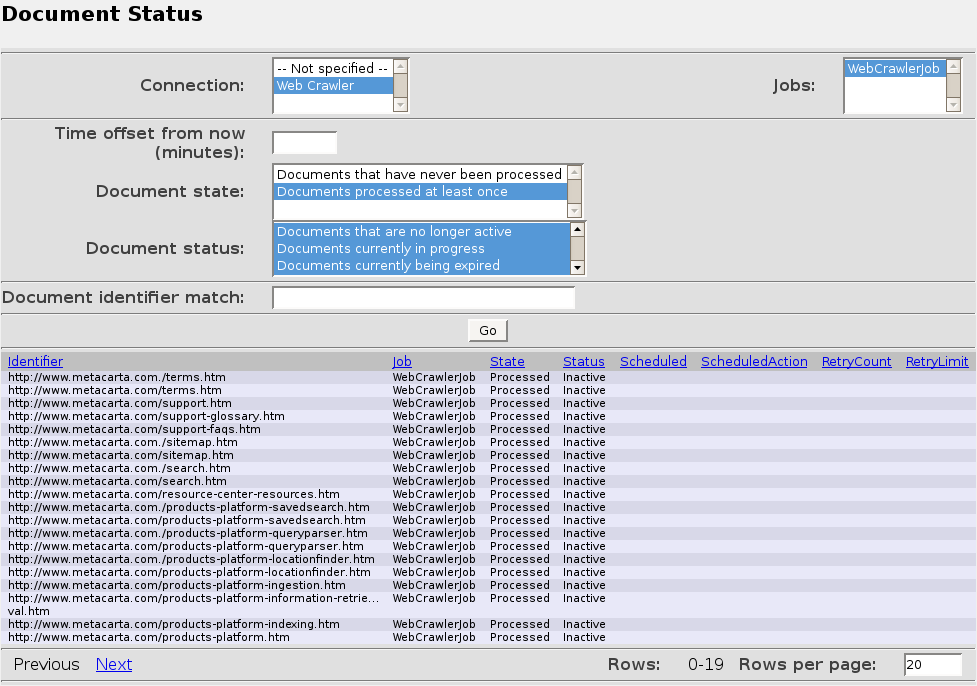
\includegraphics[width=300pt]{web-document-report}

\begin{itemize}

\item \textbf{Connection:} The repository connection from which to 
generate a report. You must select the repository connection and click
Continue to see all repository-specific options. %Are there any?

\item \textbf{Time offset from now:} Defaults to zero. Allows you to
see estimates of future status or, with negative numbers, a record of
past status.

\item \textbf{Document state:} Allows you to select documents that
have not yet been processed or documents that have been processed
at least once.

\item \textbf{Document status:} Allows you to choose one or more 
statuses of document to report on. The statuses you can choose are:

\begin{itemize}

\item Documents that are no longer active

\item Documents currently in progress

\item Documents currently being expired

\item Documents currently being deleted

\item Documents currently available for processing

\item Documents currently available for expiration

\item Documents not yet processable

\item Documents not yet expirable

\end{itemize}

\item \textbf{Document identifier match:} A regular expression
allowing you to see only certain document identifiers. A document's
identifier is its URL.

\item \textbf{Jobs:} The job or jobs for which you want to generate
a report.

\end{itemize}

You can sort this report by any of the returned fields; to do so,
click the field names.

\subsubsection{Queue Status}

This report was generated by selecting ``Web Crawler,'' selecting both
document states, selecting all possible document statuses, clicking
continue, selecting ``WebCrawlerJob,'' and clicking Go.

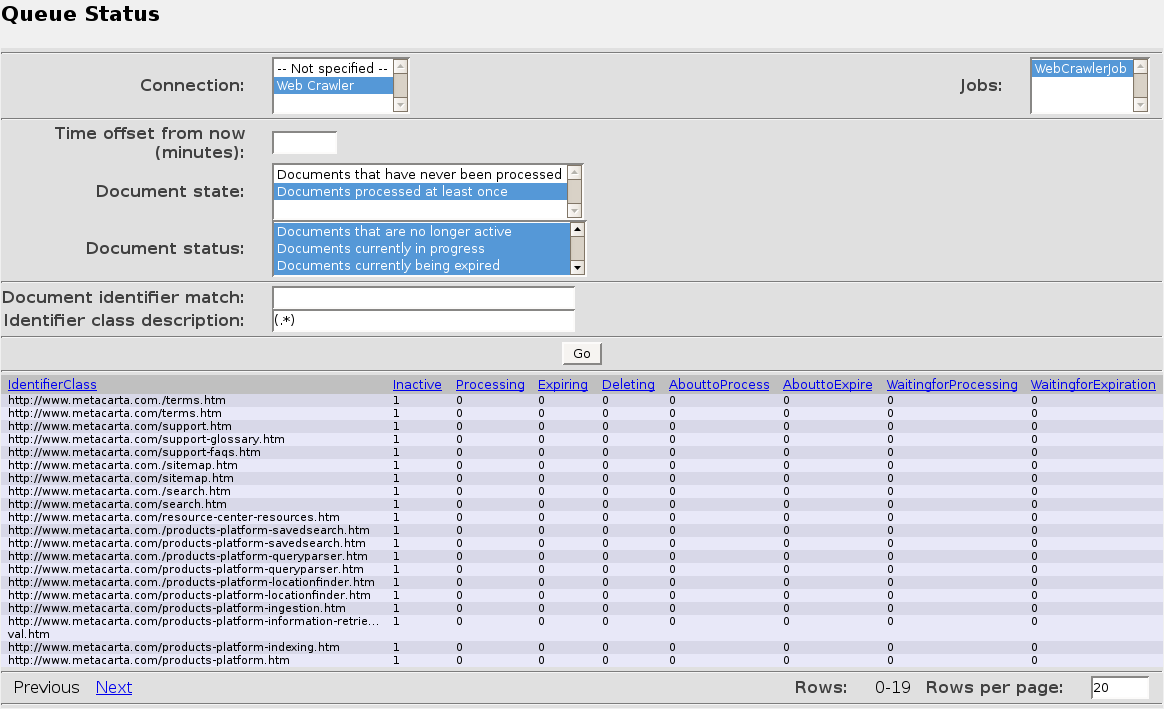
\includegraphics[width=300pt]{web-queue-report}

This form offers the same fields as the Document Status report with
one addition, the \textbf{Identifier class description}, which allows
you to group results based on a regular expression. In this case, the
identifier class description is just ``.*''. Each document is shown
individually as a group of one. If we set the identifier class
description to
\texttt{\^{}https?://([\^{}$\backslash\backslash\backslash$?/]*)},
documents would be grouped together if their URLs specified the same
server, and each group's documents would be analyzed separately from
the other documents selected. The ungrouped documents would be all
analyzed together in the first row of the results table.

\subsection{History Reports}

The four types of history report are:

\begin{itemize}

\item Simple History, which lets you list an ordered set of log events
based on chosen criteria

\item Maximum Activity, which lets you see the period of time in
which a certain event happened most often

\item Maximum Bandwith, which lets you see the period of time in
which the most bandwidth was used 

\item Result Histogram, which provides log information that would be
appropriate for constructing a histogram or other diagram

\end{itemize}

Each of these reports allows you to specify a connection, one or more
activities, a start time, an end time, an entity match, and a result code
match.  Some also allow you to specify an identifier class description
and a sliding window size. This section will show sample results for
each type of report and an explanation of the fields selected.

\subsubsection{Simple History}

This report was generated by selecting ``Web Crawler,'' 
clicking Continue, selecting ``document ingest,'' and clicking Go.

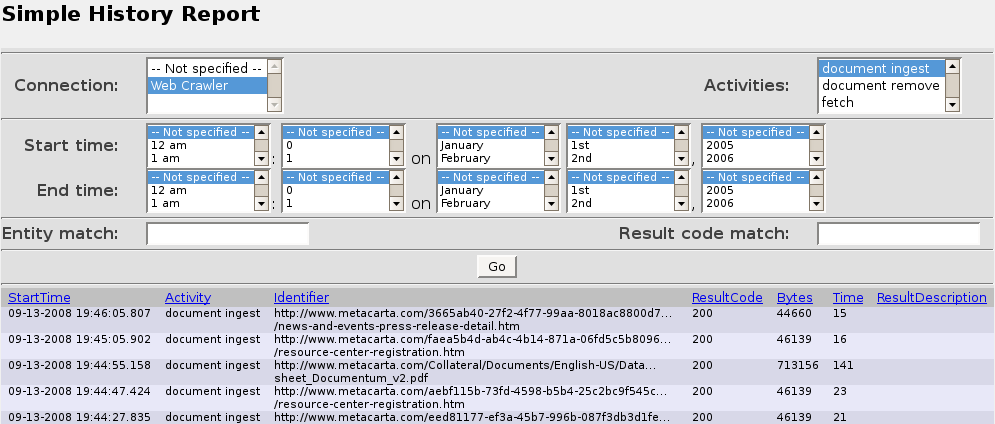
\includegraphics[width=300pt]{web-simple-history-report}

\begin{itemize}

\item \textbf{Connection:} The repository connection from which to generate
a report.

\item \textbf{Activities}: What crawler activities you would like to
see.  Your options are document ingest, document remove, fetch, job
abort, job continue, job end, job start, and job wait.

\item \textbf{Start time}: The earliest time in the crawler logs to be
considered for this query.  Choose ``Not specified'' for any field to
start at the beginning of the crawler's logs.

\item \textbf{End time:} The latest time in the crawler logs to be
considered for this query. Choose ``Not specified'' for any field 
to end at the current time.

\item \textbf{Entity match:} A regular expression to limit the
Identifier field. For the Web Crawler, the document identifiers are
the document URLs. If the entity match field in the example above had
been \texttt{www.example.com}, only document fetches with URLs from
that server would be shown.

\item \textbf{Result code match:} A regular expression to limit the
ResultCode field.

\end{itemize}

You can sort the history report by any of the returned fields; to do so,
click the field names.

\note{If you are not familiar with regular expressions,
there are a variety of tutorials available on the web,
including \url{http://gnosis.cx/publish/}\linebreak
\url{programming/regular_expressions.html} and
\url{http://perldoc.}\linebreak\url{perl.org/perlrequick.html}. If you
still have difficulty with these settings, please contact Customer Support
(see page \pageref{SupportContact}).}

\subsubsection{Maximum Activity}

This report was generated by selecting ``Web Crawler,''
clicking Continue, selecting ``document ingest,'' changing the Identifier
class description, and clicking Go.

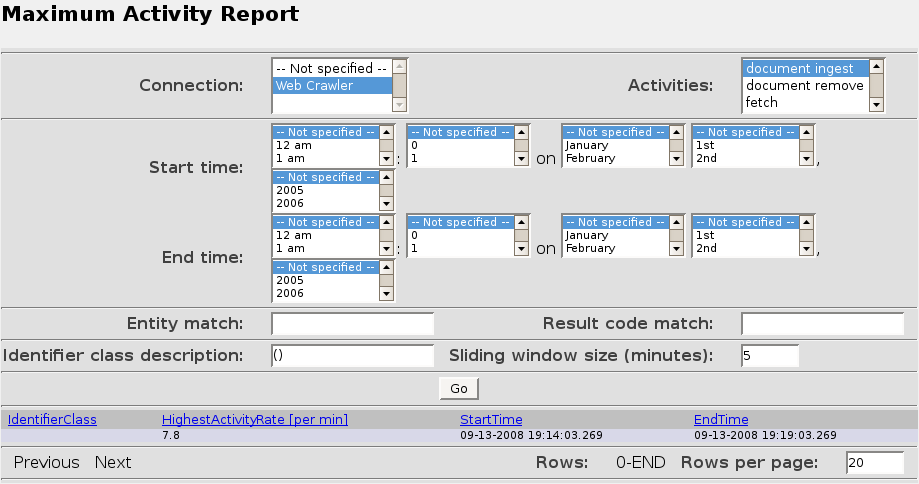
\includegraphics[width=300pt]{web-maximum-activity-report}

This form offers two more fields than the previous form:

\begin{itemize}

\item \textbf{Identifier class description:} A regular expression that
determines how to group identifiers together. The setting in the example,
\texttt{()}, groups all documents together. Some other possibilities:

\begin{itemize}

\item \texttt{(.*)}: No groupings, all ingestions listed separately.

\item \texttt{(www.example.com)}: One group of documents whose URLs contain ``www.example.com,'' a second group of documents whose URLs do not contain ``www.example.com.''

\item \texttt{\^{}http://([\^{}$\backslash\backslash\backslash$?/]*)}:
Groups for each separate server.

\item
\texttt{$\backslash$.html?($\backslash$?|\$)|$\backslash$.pdf?($\backslash$?|\$)}
One group of files with the extention ``.html'' or ``.htm'', one group
or files with the extension ``.pdf'', and one group of all other
files.


\end{itemize}

\item \textbf{Sliding window size}: The search interval in minutes.

\end{itemize}

The report returned will have only one result per group with one or more
documents in it, if there is a clear highest activity rate, or a list of
all the results tied for highest activity rate if there are more than one.

\subsubsection{Maximum Bandwidth}

This report was generated by selecting ``Web Crawler,''
clicking Continue, selecting ``document ingest,'' changing the Identifier
class description, and clicking Go.

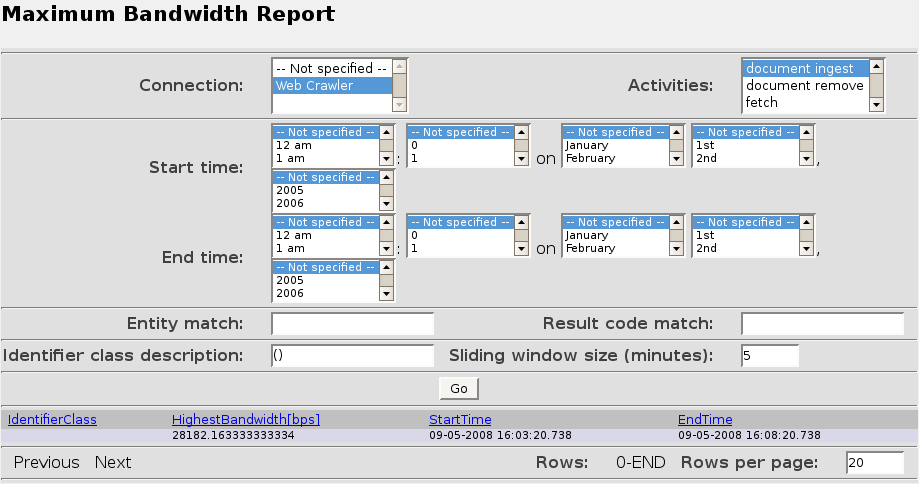
\includegraphics[width=300pt]{web-maximum-bandwidth-report}

This form offers the same fields as the maximum activity form, and
returns similar results; instead of tracking events per time window,
it tracks the window with the highest average bandwith usage, measured
in bytes per second. Again, the identifier class description has been
changed to a regular expression that will match all identifiers (and
thus in this case all documents).

\subsubsection{Result Histogram}

This report was generated by selecting ``Web Crawler,'' clicking Continue, selecting ``document ingest,''
altering the identifier class description to group documents into
groups based on server, and clicking Go.

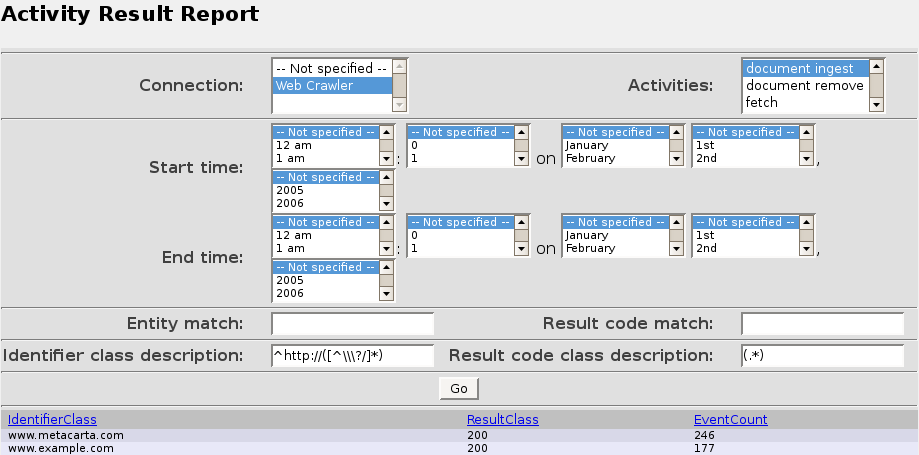
\includegraphics[width=300pt]{web-activity-result-report}

This form adds one new field:

\begin{itemize}

\item \textbf{Result code class description:} A regular expression that
determines how to group result classes together; like Identifier class
descriptions but for result classes.

\end{itemize}

This report does not produce an actual histogram, but provides data that
could be used to generate histograms.  

\end{changemargin}
